\section{Introduction}

The recent development in electric circuit rapid prototyping tools, such as ink-based electrical circuitry allows users to prototype without wiring. Unfortunately, ink-based electrical circuitry is inherently difficult to modify, because electronic components are affixed on a piece of paper or board by soldering or taping. A hard-to-modify prototyping tool slows makers down due to component reattachment to a new printed circuitry. We therefore argue that the process of how circuit rapid prototyping is used for quick modification is not yet optimal.

% In other disciplines, such as in user interface design, designers achieve a fast and efficient process by iterating from low-fidelity prototyping techniques to high-fidelity techniques.

In order to allow makers to iterate quickly, hard-to-modify techniques, such as sketching and paper prototyping, give priority to speed over functionality. This trade-off pays off in the early phases of design because it encourages the quick exploration of several versions before committing further resources, eventually leading to a better design.
\begin{figure}
  \begin{center}
  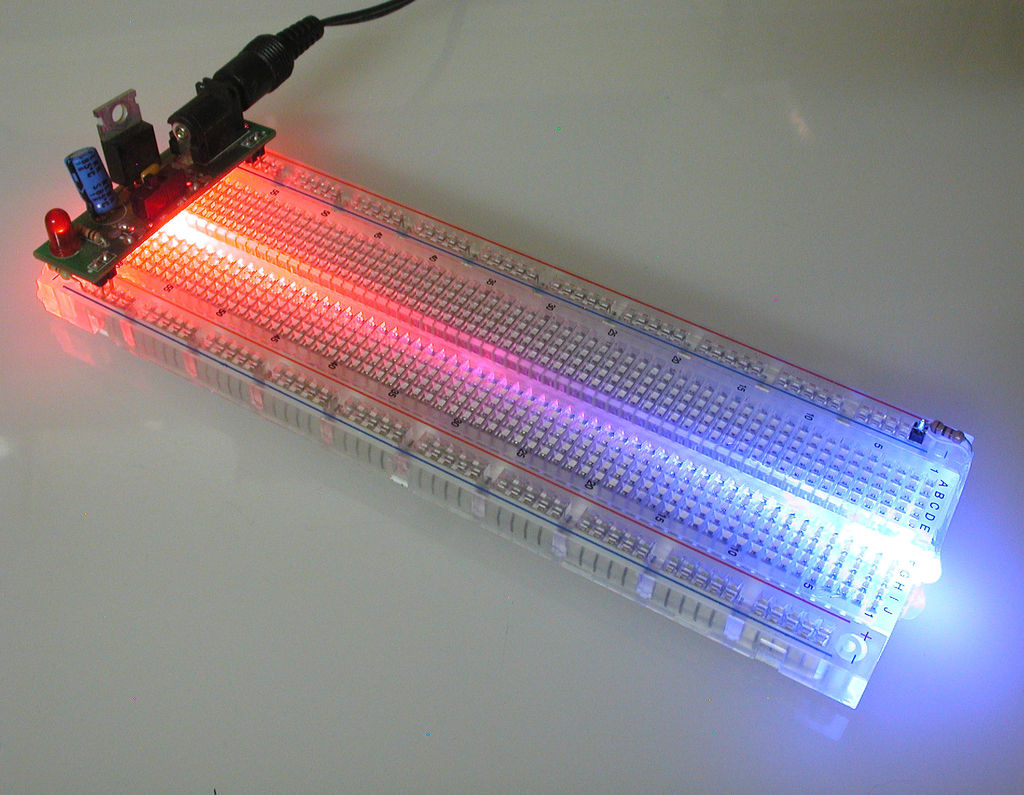
\includegraphics[width=1\columnwidth]{figures/Figure1.jpg}
  \caption{\papertitle\ is a reconfigurable perfboard for fast circuit prototyping.}
  \label{fig:FIGURE1}
  \end{center}
\end{figure}
\begin{figure}
  \begin{center}
  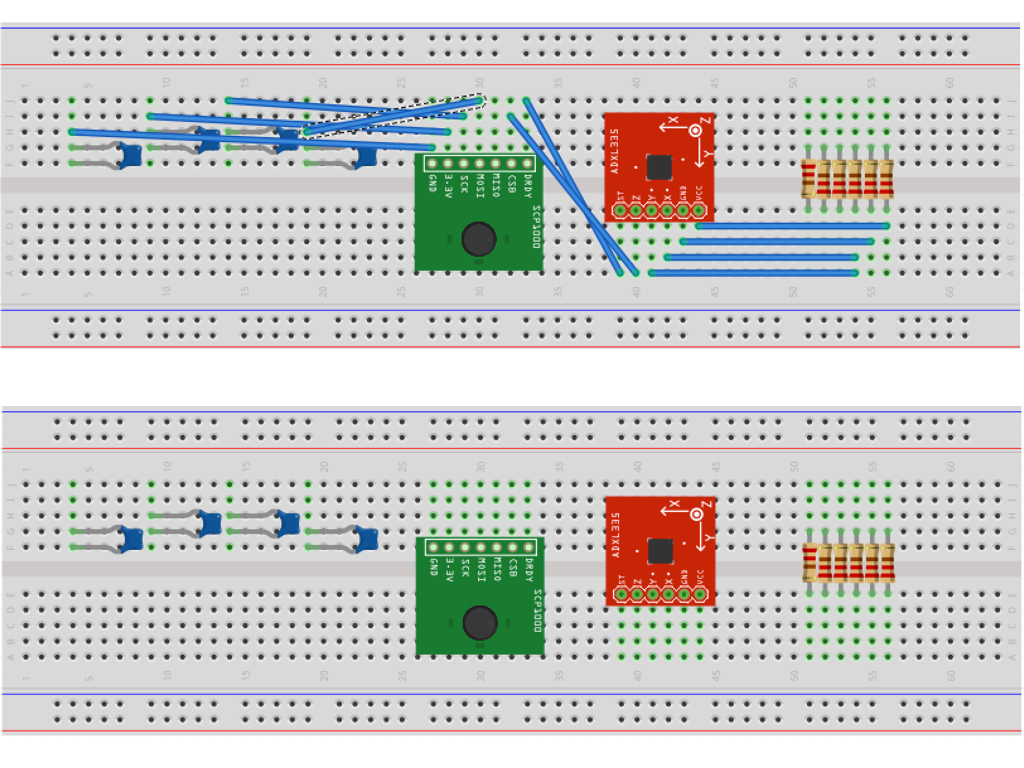
\includegraphics[width=1\columnwidth]{figures/current.jpg}
  \caption{Compared with current circuit prototyping, \papertitle enables easy and reusable fast prototyping without any wires and soldering.}
  \label{fig:FIGURE5}
  \end{center}
\end{figure}
We argue that the same principle should apply to circuit prototyping – a concept we call easy-to-modify circuit prototyping. In contrast to the traditional workflow, in which the circuit prototyping is always done as time-consuming soldering or hard-to-modify ink-based techniques, easy-to-modify prototyping makes all intermediate versions as fast and easy-to-modify circuits. Only at the end, when the design is finished, the complete circuit prototype is printed as PCB (Figure 2).

One ink-based circuit prototyping approach is Inkjet — a system that prints circuits speed-up by substituting wires with conductive silver ink. Unfortunately, Inkjet requires users to attach components on the circuit with hard-to-modify approaches, such as taping or soldering.

In this paper, we present a easy-to-modify approach that not only save time, but also save the cost of components. The key idea is to combine the mechanism of breadboard and ink-based circuit printing to provide an easy-to-modify and robust approach for circuit prototyping , i.e. a 3D print in which surfaces have been replaced with a wireframe mesh. Our approach runs on both standard FDM 3D printers, such as the PrintrBot or the Kossel mini (rather than on a 5 axis robot arm [12]) and Inkjet printers (Brothers MFC)—users only need to install the uCirKit software. Resin-coated photo paper helps to maximize the conductivity of the printed wires.
